\chapter{Разработка программных модулей системы электронного обучения и результаты экспериментов} \label{chapt4}

\section{Архитектура системы электронного обучения на основе онтологий} \label{sect4_1}

Для реализации описанных алгоритмов, методов и методик была разработана система электронного обучения ECOLE (Enhanced Course Ontology for Linked Education). Кроме основных функций системы электронного обучения ECOLE выполняет функции семантического агрегатора открытых образовательных ресурсов.

Основными функциями системы ECOLE являются:

\begin{itemize}
\item сбор учебных материалов из внешних источников и преобразование их в структурированный формат;
\item предоставление данных пользователям в различных форматах (текст, графика, мультимедиа);
\item предоставление данных сторонним приложениям по работе с Linked Data (SPARQL-endpoint);
\item возможность редактирования и создания новых учебных материалов и изменение образовательных процессов;
\item связывание учебных материалов со сторонними источниками (электронные библиотеки, мультимедиа ресурсы, социальные сети);
\item анализ актуальности учебных материалов и курсов (обновление данных полученных из внешних источников);
\item анализ полноты и сбалансированности учебных материалов (покрытия модуля тестами, рейтинговая система оценки материалов);
\item поиск учебных материалов;
\item разграничение доступа к редактированию информации различным группам пользователей.
\end{itemize}

Сервер системы электронного обучения ECOLE основан на платформе Information Workbench. Платформа Information Workbench предоставляет функционал для работы с открытыми связными данными Linked Open Data. Платформа основана на использовании программных модулей с открытым исходным кодом. Пользовательский интерфейс сервера ECOLE основан на модуле семантической разметки Semantic MediaWiki. Данный модуль позволяет использовать переопределенные шаблоны и визуальные средства для отображения семантических данных в виде Wiki-страниц. Редактирование и управление RDF данными системы реализовано с использованием платформы OpenRDF Sesame. Сервер системы ECOLE поддерживает запросы SPARQL. Сервер предоставляет открытую точку доступа для SPARQL запросов.

Внешним интерфейсом системы электронного обучения ECOLE является облегченная система управления образованием Learning Management System (LMS). LMS предназначена для удобного представления учебных материалов пользователям системы. LMS обладает локальным хранилищем и производит управление пользовательскими данными, настройками и результатами обучения студентов. Внешний интерфейс системы предоставляет функционал по администрированию системы и управлению доступом к данным системы. В LMS реализованы модули для отображения видео-лекций, слайдов, тестов и практических заданий.

Внешний интерфейс взаимодействует с сервером системы с помощью запросов к открытой точке доступа SPARQL. Внешний интерфейс получает с сервера данные по учебным материалам и отношениям между объектами курса. Приватные персональные данные пользователей и настройки LMS хранятся в локальной памяти внешнего интерфейса.

Общая архитектура системы электронного обучения ECOLE представлена на рисунке \ref{img:overall_arch}.

\begin{figure} [h] 
  \center
  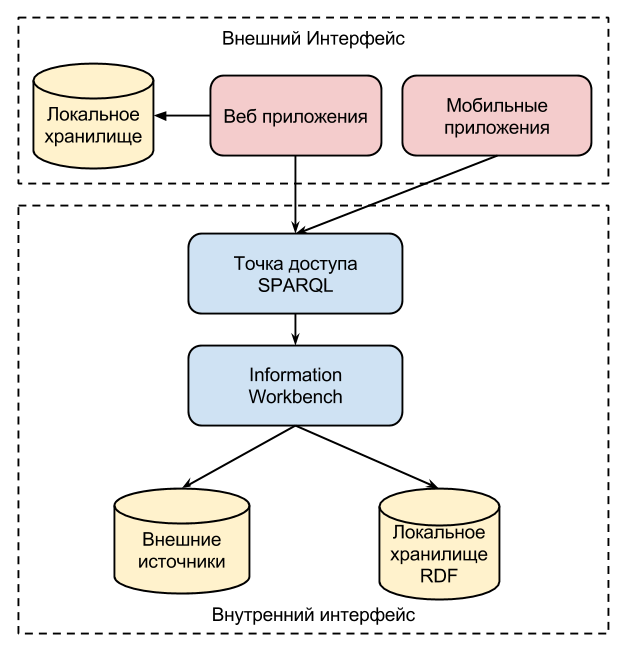
\includegraphics [scale=0.6] {overall_arch}
\caption{Общая архитектура системы электронного обучения ECOLE.}
  \label{img:overall_arch}  
\end{figure}

LMS реализована на языке Python с использованием Django Web Framework  \cite{holovaty2009definitive}. Библиотека SPARQLWrapper использована отправки запросов к точке доступа SPARQL. Когда пользователь завершает тест, LMS собирает результаты теста, ответы на задания и дополнительную статистику и записывает полученные данные на сервер с помощью запроса SPARQL Update Query \cite{seaborne2008sparql}. В результате прохождения теста студентом на сервере создается объект класса <<AttemptToPassTest>> (Попытка) с набором правильных и неправильных ответов на задания теста. Данный объект связывается с объектом студента. В целях безопасности персональных данных объекты студентов идентифицируются с использованием хеш-суммы электронной почты студента.

После прохождения теста система предоставляет студенту информацию о количестве и доле правильных ответов на задания теста. Так же студенту предоставляется список концептов предметной области для повторения. Система генерирует список проблемных концептов для студента, используя результаты теста и связи между концептами системы и заданиями теста. Для каждого концепта предметной области, связанного с заданиями теста, производится расчет рейтинга на основе ответов студента. Лист проблемных концептов сортируется в порядке возрастания рейтинга. Чем выше рейтинг концепта, тем больше правильных ответов дал студент на задания связанные с данным концептом и тем меньше затруднений вызвал у студента данный концепт. Рейтинг концепта, полученный в контексте прохождения теста, может быть отражен в глобальном рейтинге знаний концептов студентом. Глобальный рейтинг знаний для каждого концепта позволяет студенту выявлять проблемные концепты и восполнять знания по ним.   


\section{Описание пользовательских интерфейсов разработанной системы электронного обучения} \label{sect4_2}

%%%%%%%

%% СКРИНШОТЫ И ОПИСАНИЕ СИСТЕМЫ















%%%%%%%

\section{Метод преобразования онтологий системы электронного обучения в формат SCORM} \label{sect4_3}

Учебные материалы хранящиеся в семантическом формате не могут быть интегрированы системы электронного обучения без поддержки семантических технологий. Данный факт не позволяет системе ECOLE экспортировать агрегированные учебные материалы в окружение сисем электронного обучения университетов. В данный момент существуют стандарты позволяющие интегрировать и обмениваться учебными материалами между системами электронного обучения. Одним из таких стандартов является стандарт SCORM. Для реализации конвертации и экспорта учебных материалов из семантического формата в формат SCORM был разработан программный модуль преобразования. Экспортирование данных из системы ECOLE в формат SCORM позволит интегрировать учебные материалы в большое количество типов систем электронного обучения, поддерживающих стандарт SCORM. Одной из таких систем является популярная ситсема электронного обучения Moodle.

Разработанный модуль решает следующий ряд задач:

\begin{itemize}
\item извлечение данных в семантических форматах из ситсемы электронного обучения на основе семантических технологий;
\item создание учебных материалов из извлеченных данных по предопределенным шаблонам;
\item генерация данных из учебных материалов в соответствии со стандартом SCORM;
\item поддержка различных интерфейсов управления модулем, таких как  пользовательский интерфейс или REST API.
\end{itemize}

Разработанный модуль использует сервисы и программные модели платформы Information Workbench. В основе модуля лежит Сервис Преобразования SCORM. Данный сервис взаимодействует с различными модулями сервера и интерфейс системы ECOLE для извлечения учебных материалов и их преобразования в формат SCORM. Модуль реализован на языке Java и интегрирован в платформу Information Workbench. Архитиктура программного модуля представлена на рисунке \ref{img:overall_scorm_arch}.

\begin{figure} [h] 
  \center
  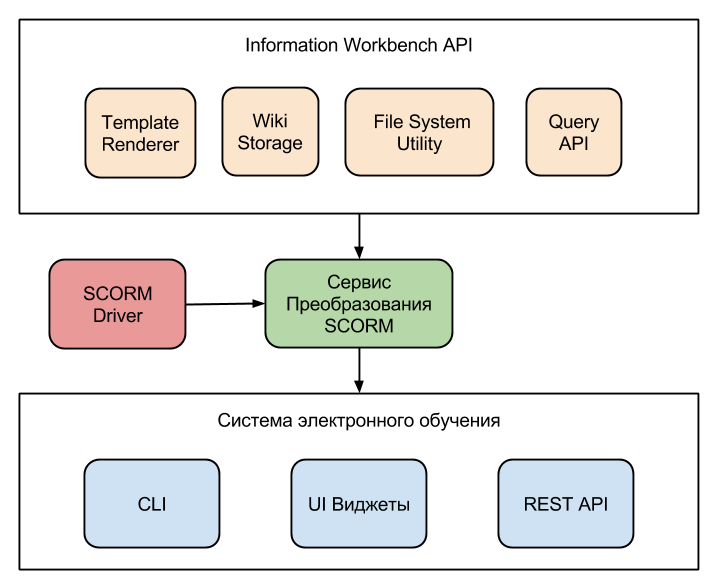
\includegraphics [scale=0.65] {overall_scorm_arch}
\caption{Архитектура программного модуля преобраования данных в формат SCORM в системе ECOLE.}
  \label{img:overall_scorm_arch}  
\end{figure} 

Сервис Преобразования SCORM использует модуль Query API для сбора семантических данных. Для сбора предопределенных шаблонов используется сервис Wiki Storage. Программный модуль Template Renderer используется для генерации HTML страниц из собранных учебных материалов по преопределенным шаблонам. File System Utility используется для управления файлами и директориями системы. Для генерации данных в формате SCORM используется внешняя библиотека SCORM Driver. В качестве интерфейса Сервиса Преобразования SCORM могут выступать пользовательские <<виджеты>>, REST API и интерфейс командной строки (CLI).


Метод преобразования учебных материалов в формат SCORM заключается в формировании набора HTML страниц на основе шаблонов и семантических данных. Для создания SCORM пакета необходимы следующие шаблоны:

\begin{itemize}
\item шаблон начальной страницы электронного курса;
\item шаблон лекции;
\item шаблон заключительной страницы электронного курса.
\end{itemize}

При генерации каждный шаблон получает информацию о соответсвующем объекте онтологии. Шаблоны начальной и заключительной страницы курса получают информацию об объекте электронного курса. Шаблон лекции получает информацию об объекте лекции электронного курса. В результате генерации формируются HTML страницы с данными переданных объектов. Алгоритм преобразования семантически данных учебных материалов в формат SCORM представлен на рисунке \ref{img:overall_scorm_algo}.

\begin{figure} [h] 
  \center
  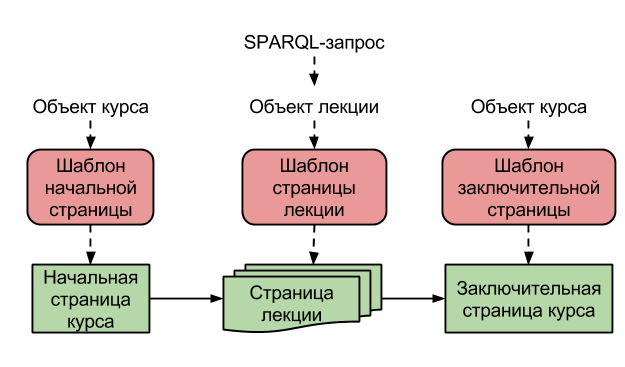
\includegraphics [scale=0.7] {overall_scorm_algo}
\caption{Алгоритм преобразования семантически данных учебных материалов в формат SCORM.}
  \label{img:overall_scorm_algo}  
\end{figure} 

Данные об объектах собираются с помощью запросов SPARQL. Шаблоны описываются с помощью синтаксиса Semantic MediaWiki. Шаблоны поддерживают разметку HTML. В ходе генерации учебных материалов в формате SCORM Сервисом Преобразования SCORM  производиться дополнительное наполнение заголовков HTML страниц и извлечение медиа ресурсов из содержания учебных материалов. Ниже представлен пример описания шаблона  лекции для разработанного программного модуля. 

\begin{lstlisting}
= $this.rdfs:label$ =

=== About ===

'''Module''': $this.learningRu:isLectureOf$
'''Number of lecture''': $this.learningRu:numberOfLecture$ 

=== Terms ===

{{#sparql: SELECT DISTINCT ?label
 WHERE { ?term learningRu:isTermOf {{this}} . 
 ?term rdfs:label ?label } } 
 | format=template  | template=Template:ListTemplate}}

\end{lstlisting}

Разработанный программный модуль позволяет преподавателям и авторам экспортировать из системы ECOLE электронные курсы в формат SCORM для дальнейшей интеграции в другие системы электронного обучения. 

\section{Результаты применения методики агрегации данных в системе электронного обучения} \label{sect4_4}

Основной набор данных системы электронного обучения ECOLE формировался вручную. Часть данных была создана с помощью разработанных методик, методов  и алгоритмов наполнения и гармонизации онтологии. Набор данных системы электронного обучения на основе семантических технологий состоит из объектов образовательного процесса, таких как курс, модуль, лекция, тест, практика, концепт, предметная область и книга. Статистика по количеству объектов в наборе данных системы электронного обучения ECOLE приведена в таблице  \ref{table:nlp_resutls}.

\begin{table}[h!]
\centering
\caption{Количество объектов в наборе данных системы электронного обучения ECOLE.)}
\label{table:dataset_num}
\begin{tabular}{ |p{9cm}|c|  }
\hline Электронные курсы & 4 \\
\hline Модули & 14 \\
\hline Лекции & 90 \\
\hline Тесты & 4 \\
\hline Предметные области & 8 \\
\hline Концепты & 587 \\
\hline Концепты, связанные с объектами DBpedia & 219 \\
\hline Книги & 4094 \\
\hline Книги из учебных материалов Университета ИТМО & 1131 \\
\hline Книги из электронной библиотеки BNB & 2951 \\
\hline
\end{tabular}
\end{table}


В результате работы NLP алгоритмов по извлечению концептов из тестов были получены результаты, представленные в таблице \ref{table:nlp_resutls}. С одной стороны с концептами было связано 95\% заданий тестов. С другой стороны более 50\% концептов курса остались не связанными с заданиями тестов. Одной из причин данного явления является косвенное употребление концептов предметной области в задании. Чтобы решить такое задание необходимо знать концептов, который не упомянут ни в тексте задания, ни в тексте ответов. Примером таких заданий является следующая задача.

\begin{verbatim}
Длина лестницы - 5 метров. На каком растоянии от основания 
стены необходимо поставить данную лестницу, чтобы пересечь
стену длиной 4 метра. 
Дайте свой ответ в метрах с точностью до одного знака после запятой.
\end{verbatim}


Примером таких заданий являются задачи на поиск длинны гипотенузы треугольника при известных катетах. Косвенно связанным концептом предметной области в данном примере является термин <<Теорема Пифагора>>. В текущей реализации метода извлечение косвенных концептов не производится. В будущем планируется использование семантических связей между концептов для выявления косвенных концептов предметной области в заданиях тестов.

\begin{table}[h!]
\centering
\caption{Результаты работы алгоритмов обработки естественного языка по извлечению концептов предметной области из тестов.)}
\label{table:nlp_resutls}
\begin{tabular}{ |p{12cm}|c|  }
\hline Количество обработанных заданий & 20 \\
\hline Процент связанных заданий, \% & 95 \\
\hline Процент несвязанных заданий, \% & 5 \\
\hline Количество извлеченных концептов-кандидатов & 155 \\
\hline Количество концептов извлеченных вручную & 30 \\
\hline Концепты системы, совпавшие с концептами-кандидатами, \% & 50 \\
\hline Концепты-кандидаты, совпавшие с концептами системы, \% & 8 \\
\hline Концепты-кандидаты, добавленные в систему после прохождения проверки, \%  & 6 \\
\hline Ложные концепты-кандидаты, \% & 86 \\
\hline
\end{tabular}
\end{table}  


\section{Результаты применения методов анализа на учебных курсах и группах студентов} \label{sect4_5}

Модуль автоматического расчета оценки и рейтинга знаний студента по концептам и предметным областям был разработан на языке Python и интегрирован в систему электронного обучения ECOLE с использованием Django Web Framework. Работа модуля была применена при прохождении студентами курса <<Интеллектуальные системы>>. В результате работы модуля было рассчитано значение для концептов из предметной области <<Экспертные системы>>. В данный момент в предметной области содержится 43 концепта. Десять концептов с наибольшим значением представлены в таблице \ref{table:term_importance_result}. Полученные результаты демонстрируют значимость концептов предметных областей в образовательном процессе. Для изучения концептов одной предметной области могут потребоваться знания концептов другой предметной области. Таким образом, значимость концептов не зависит от предметных областей, к которым данные концепты относятся. Расчеты показывают, что базовые понятия в предметной области не являются самыми важными в ней.    

\begin{table}
\centering
\caption{Значения концептов предметной области <<Экспертные системы>>}
\label{table:term_importance_result}
\begin{tabular}{|p{7cm}|c|}
\hline Концепт & Значение \\
\hline Инженерия знаний & 3.749703 \\
\hline Знания & 1.796706 \\
\hline Извлечение знаний & 1.796706 \\
\hline Рабочая память & 1.706427 \\
\hline Представление (репрезентация) знаний & 1.606853 \\
\hline Процесс разрешения конфликтов & 1.374309 \\
\hline Язык представления знаний & 1.191552 \\
\hline Экстенсионал & 1.169817 \\
\hline Интенсионал & 1.169817 \\
\hline Интуитивные знания & 1.169817 \\
\hline
\end{tabular}
\end{table}

При прохождении студентом  лекций и тестов модуль рассчитывает рейтинги концептов и предметных областей в соответствии с разработанными методами. В результате студенту демонстрируется список предметных областей и концептами с оценками. Интерфейс списка оценок представлен в приложении  \ref{APP_D_STUD_KNOW_TOTAL}.

В ходе эксперимента в системе электронного обучения ECOLE были собраны статистические данные по действиям студентов. Более 250 студентов прошли электронный курс <<Интеллектуальные системы>>. На основе полученных данных и разработанных методов системой был построен анализ учебных материалов и действий студентов в системе. Так же на основе разработанного алгоритма оценки знаний студентом концептов и предметных областей был произведен расчет рейтингов знаний по предопределенным показателям. 

Для сравнения результатов системы с представлением студентов и автором были произведены опросы. В опросе для студентов содержалось 5 вопросов о личном мнении студентов по содержанию электронного курса и их собственным знаниям. В опросе приняло участие 43 студента. В опросе были заданы следующие вопросы:

\begin{itemize}
\item Какие 5 концептов предметной области являются самыми сложными для вас?
\item Какие 5 концептов предметной области вы знаете/понимаете лучше всего?
\item Какие 3 концепта предметной области термина являются самыми важными в курсе?
\item Какая из лекций показалась вам наиболее объемной?
\item Изучение какой лекции позволило вам ответить на большее количество вопросов?
\end{itemize}

Для ответов на описанные вопросы студентам предоставлялись варианты ответов. Варианты ответов покрывали полный набор возможных объектов курса, соответствующих заданному вопросу.

Для сравнения мнения системы и авторов электронных курсов был произведен дополнительны опрос авторов. Авторами курса являются эксперты в предметной области задействованные при составлении электронного курса. В опросе для авторов содержалось 4 вопроса о мнении авторов по содержанию электронного курса. В опросе приняло участие 4 автора. В опросе были заданы следующие вопросы:

\begin{itemize}
\item Укажите 10 самых сложных концептов электронного курса и расположите их в порядке от 1 до 10 по возрастанию сложности.
\item Укажите 10 самых важных концептов электронного курса и расположите их в порядке от 1 до 10 по возрастанию сложности.
\item Пронумеруйте лекции в порядке возрастания их объема. 
\item На сколько процентов курс покрыт тестами?
\end{itemize}

Для ответов на описанные вопросы авторам были предложены варианты ответов. Для оценки покрытия курса тестами вариантов ответов не предоставлялось. 

На основе полученных данных системы и данных опросов был произведен копмлексный анализ электронного курса. Анализ производился с целью выявления недостатоков в содержании, структуре электронного курса и подачи учебных материалов.

В начале была произведена оценка объема лекций и покрытия лекций тестами в электронном курсе. Система оценивала объем лекций на основе количества связанных концептов предметной области. Данный подход позволяет оценивать учебные материалы не на основе их структуры или объема, а на основе их содержания. Покрытие лекций тестами расчитывалось системой на основе анализа количества концептов лекции использованных в тестах. Полученные результаты представлены в диаграммах в приложении \ref{APP_E_COVER}. В диаграммах демострируется отношение показаний системы к средней оценке по опросам авторов и студентов. Совпадения оценок студентов и системы в результах покрытия лекций показывает, что система может оценивать и выявлять те лекции курса, которые будут самыми позлезными при прохождении тестов. Средняя оценка покрытия элеектронного курса тестами расчитанная системой равна 77\%. Средняя оценка покрытия курса тестами у авторов составляет 75\%. Минимальная разница между оценками свидетельствует о правильной методике расчета покрытия лекций тестами. С другой стороны оценки в результатах объемов лекций различааются. Это объясняется тем, что авторы и студенты оценивают объем лекций по их сруктуре, а не по смысловому содержанию. В данном эксперименте система выявила недостатки электронного курса в виде плохой сбалансированности изложения учебных материалов.      


Для оценки проблемных концептов предметной области в электронном курсе использовался анализ ответов студентов на вопросы тестов, связанных с определенными концептами. Далее в системе производился отношения правильных ко всем ответами студентов на вопросы связанные с определенным концептом. На основе аналитических данных системы и данных опросов студентов и авторов был произведен сравнительный анализ. Полученные результаты представлены в диаграммах в приложении \ref{APP_E_PROBLEM}. Всего в опросе студентов в качетсве проблемных концептов было упомянуто 75\% всех концептов системы. Полученные результаты показывают полное не совпадение оценок системы, авторов и студентов. Данный факт указывает на то, что авторам круса необходимо пересмотреть и улучшить изложение учебного материала по выявленным системой проблемным концептам. Разница между оценкой студентов и показаниями системы обуславливается тем, что студенты часто не могут выявить наиболее проблемные для себя концепты предметной области.

Для оценки значимости концептов предметной области в электронном курсе использовался анализ зависимостей между концептами и их потомками. Система производила расчет значимости для каждого концепта на основе разработанного метода. На основе аналитических данных системы и данных опросов студентов и авторов был произведен сравнительный анализ. Полученные результаты представлены в диаграммах в приложении \ref{APP_E_IMPORT}. Результаты показывают 30\% совпадений в оценке системы с оценкой опросов. Всего в опросе студентов в качетсве проблемных концептов было упомянуто 50\% всех концептов системы. На онове полученных результатов было установлено, что базовые концепты предметной области не всегда являются самыми значимыми в предметной области. На основе произведенного анализа система позволила выявить концепты, на которые авторы электронного курса должны обратить особое внимание так, как точность оценки знаний полученных по учебным материалам для данных концептов может быть не высокой в силу сильно отличающихся показателей значимости у студентов, преподавателей и системы. Другими словами предложенный алгоритм позволяет отличить значимость с точки зрения структуры круса от значимости с точки зрения содержания предметной области.

В завершении эксперимента была произведена оценка знания студентами концептов и предметных областей электронного курса. Система расчитывала оценку знаний студентами концептов предметной области на основе их действий в системе электронного обучения. Расчет производился по разработанным алгоритмам используя показатели прохождения студентами теоретического материала и тестов электронного курса. Для полученных оценок знаний студентами концептов был произведен сравнительный анализ с данными опросов студентов. Среднее совпадение показаний по результатам системы и опроса составило 30\%. На основе полученных оценок система произвела расчет оценки знаний студентами предметной области <<Экспертные системы>>. Далее был произведен сравнительный анализ полученных показаний с баллами выставленными в электронный журнал для каждого студента, учавствующего в опросе. Полученные результаты представлены в диаграммах в приложении \ref{APP_E_RATE}. Из полученных результатов следует, что при 100\% оценке студента в электронном журнале значение оценки знания предметной области, полученное системой, не превышает 40\%. Это можно объяснить тем, что при прохождении электронного курса студент отвечает на вопросы связанные только с частью концептов предметной области. Существует доля концептов предметной области, знания по которым могут быть не проверены на прямую в тестах электронного курса в процессе обучения. Оценка таких концептов может быть произведена на основе анализа косвенных связей между концептами предметных областей.

%%%%%%%%%%%%%%%%%%%%%%%%
% Считай корреляцию













%%%%%%%%%%%%%%%%%%%%%%%%



Полученные результаты эксперимента позволили выявить ряд недостатков в структуре и содержании электронного курса <<Интеллектуальные системы>>. Сформированные аналитические данные позволят авторам внести изменения в учебные материалы с целью увеличения полноты и сбалонсированности курса, а так же увеличинию успеваемости студентов.

\clearpage